\subsection*{Hovedmenu} \label{sec:MVCHovedmenu}
Hovedmenuen er den primære grænseflade, der inddeles i en boundary samt en tilhørende controller. Disse fremgår af \autoref{fig:Designhovedmenu}.

\begin{figure} [H]
\centering
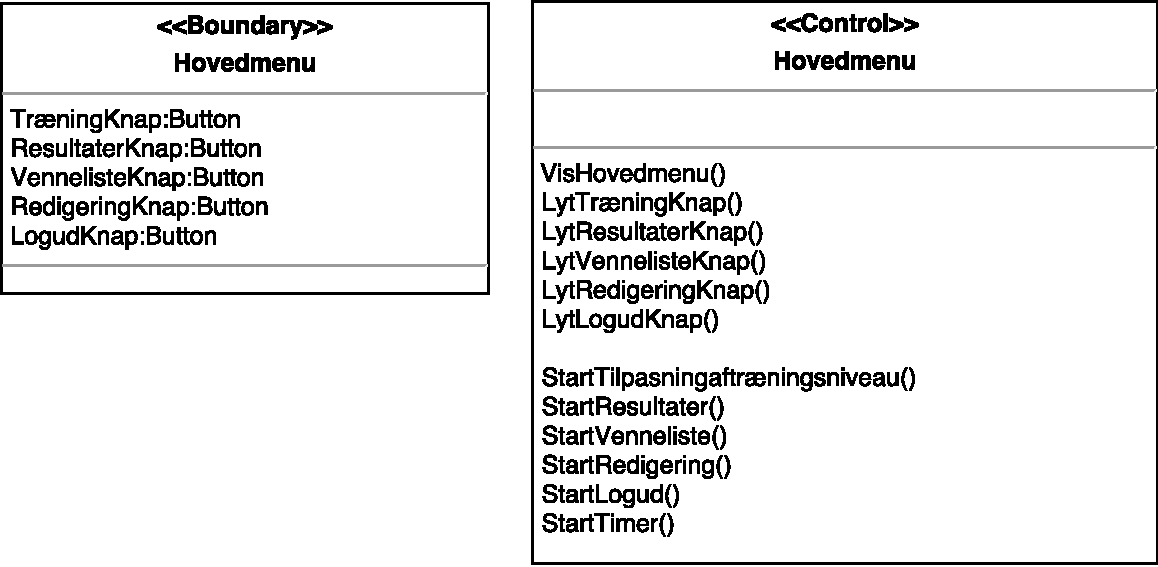
\includegraphics[width=0.9\textwidth]{figures/MVC/MVCHovedmenu}
\caption{Designklasser for hovedmenu.}
\label{fig:Designhovedmenu}
\end{figure}

\noindent
\textit{HovedmenuGrænseflade} skal tillade adgang til de forskellige funktionaliteter af app’en, herunder skal det være muligt at tilgå træning, resultater, venneliste, redigering samt log ud. Funktionaliteterne tilgås via tilhørende knapper af typen button. 

Til grænsefladen er der ligeledes en \textit{HovedmenuController}, som viser layoutet for hovedmenuen. Controlleren lytter derudover efter de forskellige knapper, hvorefter den respektive metode startes.  
